% --- INICIO DE PLANTILLA PERSONALIZADA ---
\documentclass[oneside,11pt]{Latex/Classes/PhDthesisPSnPDF}

% --- Paquetes Originales ---
\usepackage{blindtext}
\usepackage{actuarialangle} 
\usepackage{tabularx}
\usepackage{float}
\usepackage{multirow, array}
\usepackage[usenames,dvipsnames,svgnames,table]{xcolor}
\usepackage{longtable}
\usepackage{latexsym,amsmath,amssymb,amsfonts}
\usepackage{enumitem}
\usepackage{xparse}
\usepackage{booktabs}
\usepackage[round, sort, numbers]{natbib}  
\usepackage{adjustbox}
\usepackage[utf8]{inputenc}
\usepackage{caption}
\usepackage{graphicx}
\usepackage{hyperref}
\usepackage{cleveref}

% Definición de colores
\definecolor{miblue}{RGB}{68, 114, 196}

% --- CAMBIO CRÍTICO 1: Usar \input para macros en el preámbulo ---
% \include da problemas antes del begin document. \input es seguro.
\input{Latex/Macros/MacroFile1}

% --- Definiciones de seguridad (por si la clase falla al cargar alguna variable) ---
\providecommand{\facultad}[1]{\def\lafacultad{#1}}
\providecommand{\escudofacultad}[1]{\def\elescudo{#1}}
\providecommand{\degree}[1]{\def\elgrado{#1}}
\providecommand{\director}[1]{\def\eldirector{#1}}
\providecommand{\lugar}[1]{\def\ellugar{#1}}
\providecommand{\degreedate}[1]{\def\lafecha{#1}}

% --- Configuración para bloques de código de R (Pandoc) ---

%%%%%%%%%%%%%%%%%%%%%%%%%%%%%%%%%%%%%%%%%%%%%%%%%%%%%%%%%%%%%%%%%%%%%%%%%%%%%%%%
%                         DATOS (Conectados a RMarkdown)                       %
%%%%%%%%%%%%%%%%%%%%%%%%%%%%%%%%%%%%%%%%%%%%%%%%%%%%%%%%%%%%%%%%%%%%%%%%%%%%%%%%
\title{La estadistica Vs Comunidad Pokemon}
\author{Angelo Freda \\ Stephannie labrador \\ Barbara mejía}

% Lógica para Facultad: Si la defines en el YAML la usa, si no, usa la default

\facultad{Facultad de Ciencias Económicas y Sociales \\ Escuela de
Estadistica y Ciencias Actuariales}
  \escudofacultad{Latex/Classes/Escudos/faces}

\degree{Computación I}
\director{Jesus Ochoa \\ Oliver Triveño}
\degreedate{Febrero 2026} 
\lugar{Caracas}

\portadatrue 

% Metadatos PDF
\keywords{}
\subject{}

% --- CORRECCIÓN PARA PANDOC NUEVO (Imágenes) ---
\makeatletter
\providecommand{\pandocbounded}[1]{#1}
\makeatother


%%%%%%%%%%%%%%%%%%%%%%%%%%%%%%%%%%%%%%%%%%%%%%%%%%%%%
%                   DOCUMENTO                       %
%%%%%%%%%%%%%%%%%%%%%%%%%%%%%%%%%%%%%%%%%%%%%%%%%%%%%
\begin{document}

\maketitle

%%%%%%%%%%%%%%%%%%%%%%%%%%%%%%%%%%%%%%%%%%%%%%%%%%%%%
%                  PRÓLOGO                          %
%%%%%%%%%%%%%%%%%%%%%%%%%%%%%%%%%%%%%%%%%%%%%%%%%%%%%
\frontmatter

% Puedes agregar dedicatorias desde el YAML si quieres, o dejarlas fijas aquí

%%%%%%%%%%%%%%%%%%%%%%%%%%%%%%%%%%%%%%%%%%%%%%%%%%%%%
%                   ÍNDICES                         %
%%%%%%%%%%%%%%%%%%%%%%%%%%%%%%%%%%%%%%%%%%%%%%%%%%%%%
\setcounter{secnumdepth}{3}
\setcounter{tocdepth}{3}

\tableofcontents



\cleardoublepage

  \cleardoublepage       % Empieza en página derecha (estándar en tesis)
  \chapter*{Resumen}     % Crea el título "Resumen" sin numeración (Capítulo *)
  \addcontentsline{toc}{chapter}{Resumen} % (Opcional) Lo añade al índice
  
  Resumen del trabajo de
investigación\ldots{}             % Aquí se pega el texto que escribiste en el YAML
  
  \cleardoublepage

%%%%%%%%%%%%%%%%%%%%%%%%%%%%%%%%%%%%%%%%%%%%%%%%%%%%%
%                   CONTENIDO (El Corazón)          %
%%%%%%%%%%%%%%%%%%%%%%%%%%%%%%%%%%%%%%%%%%%%%%%%%%%%%
\mainmatter
\def\baselinestretch{1.5}

% --- CAMBIO CRÍTICO 2: Aquí RMarkdown inyecta todo tu texto ---
\chapter*{Introducción}

Introducción del trabajo de investigación

\chapter{Planteamiento del Problema}

En el mundo pokemon hay diferentes tipos de ellos y se dice que ciertos
tipos son mejores para ciertas estrategias, por ejemplo se cree que los
tipo roca son muy defencivos. En las comunidades online como
reddit,twitter y foros existen afirmaciones constantes sobre los
pokemones, por ejemplo los pokemones legendarios son mas lentos, pero no
existe un estudio que confirme estas afirmaciones, con los datos de la
BD(Base de Datos) de Pokemon proporcionado por la EECA determinare si
dichas creencias son estadisticamente ciertas o solo percepciones.Existe
una desconeccion entre estudios estadisticos que tienen información
objetiva y las crencias que solo estan circulando.Esto genera un
conocimiento basado en anecdotas y no en los datos de un estudio
estadistico y esto afecta a los jugadores nuevos que intentan aprender
las estrategias en el juego y terminan tomando decisiones de estrategia
basandose en información no verificada. Si nadie utiliza buena
información verificada los jugadores novatos seguiran perdiendo batallas
por informacion que puede ser erronea. Propongo utilizar la base de
datos y mediante un analicis estadistico y comprobar algunas de dichas
creencias.Se tomaron algunas afirmaciones con sentido, se calcularan
promedios y otras distribuciones estadisticas, luego se concreta si esa
creencia la acompaña los resultados.Espero generar documento de
investigación que muestre con resultados numericos y gráficos que tan
acertada esta la comunidad en relación a los resultados. El analicis se
centrara en el contexto virtual del juego y no de manera fisica.Se
analizaran los datos de la base de datos disponibles hasta la fecha
actual y el análisis esta limitado a las generaiones de pokemon desde la
primera a la novena.El universo seran todos los pokemones y variables
existentes en la base de datos y la muestra sera dependiendo de cada
objetivo.\\

La investigación confronta las creencias de la comunidad pokémon con los
resultados estadísticos, separando los mitos de la realidad. Debido a
esto, se plantea las siguientes preguntas de investigación:\\

\textbf{1.} ¿Los pokémon legendarios son superiores estadisticamente?\\

\textbf{2.} ¿Los pokémon con mayor ataque son más lentos y los más
rapidos tienen un ataque más bajo?\\

\textbf{3.} ¿Los pokémon con doble tipo son más debiles que los tipo
puro porque tienen más debilidades?\\

\textbf{4.} Los pokémon tipo psíquico dominaban en la Generación 1,¿pero
perdieron su reinado?\\

\textbf{5.} ¿cada generación introduce pokémon más poderosos?\\

\section{Justificación}

Justificación del trabajo de investigación\\

\section{Objetivos}

\subsection{Objetivo General}
\begin{itemize}
  \item{Analizar estadisticamente la validez de creencias populares sobre pokémon desde la generación una hasta las 9.}
\end{itemize}

\subsection{Objetivos Específicos}
\begin{itemize}
  \item{Comparar a los legendarios y no legendarios con el promedio de las estadisticas más importantes.}
  \item{Comparar el promedio general de la velocidad de pokémones con la velocidad promedio de los pokemones tipo roca.}
  \item{Analizar si los pokémon de tipo puro poseen promedios de estadisticas superiores al de doble tipo.}
  \item{Evaluar la evolución de las estadisticas de los pokémon tipo psíquico desde la generación 1 hasta la 9.}
  \item{Analizar el promedio de estadisticas generales por generación, para comprobar el comportamiento de poder al rededor de las 9 generaciones.}
\end{itemize}

\section{Cobertura}

\subsection{Horizontal}

Describir la cobertura Horizontal del trabajo de investigación\\

\begin{table}[ht]
\centering
\caption{Variables consideradas} 
\resizebox{10cm}{!} {
\begin{tabular}{ccc}
  \hline
\ \ \ \ \ NOMBRE DE LA VARIABLE \\ 
  \hline
   VARIABLE 1 \\ 
VARIABLE 2\\ 
VARIABLE n\\ 
   \hline
\end{tabular}
}
\end{table}

\subsection{Vertical}

Describir la cobertura Vertical del trabajo de investigación

\section{Periodo de Referencia}

Describir la fuente y el Periodo de Referencia utilizado en el trabajo
de investigación

\section{Variables}

Describir la variable en estudio en el trabajo de investigación

\chapter{Marco Teórico}

\section{Bases Teóricas}

Resumen de las bases teoricas explicadas en el capitulo y su
importancia\\

\subsection{Definición 1}

Descripción de la definición 1\\

\subsection{Definición 2}

Descripción de la definición 2\\

\subsection{Definición n}

Descripción de la definición n\\

\chapter{Marco Metódico}

En esta sección se presentan las metodologías y/o test necesarios
relacionados con la práctica divulgada en el marco teórico, así como las
fuentes de datos.

\section{Bases metódicas utilizadas en el trabajo de investigación}

Desarrollo\\

\subsection{Item 1}

Descripción\\

\subsection{Item 2}

Descripción\\

\subsubsection{Item 2.2}

Descripción\\

\subsection{Item n}

Descripción\\

\section{Comparacion estadistica de los legendarios y los no los no
lejendarios.}\label{comparacion-estadistica-de-los-legendarios-y-los-no-los-no-lejendarios.}

\begin{table}[!h]
\centering
\caption{\label{tab:unnamed-chunk-1}Primeras 10 observaciones de Los Legendarios}
\centering
\resizebox{\ifdim\width>\linewidth\linewidth\else\width\fi}{!}{
\begin{tabular}[t]{cccccc}
\toprule
\cellcolor[HTML]{D7261E}{\textcolor{white}{\textbf{Name}}} & \cellcolor[HTML]{D7261E}{\textcolor{white}{\textbf{Type\_1}}} & \cellcolor[HTML]{D7261E}{\textcolor{white}{\textbf{Total\_Stats}}} & \cellcolor[HTML]{D7261E}{\textcolor{white}{\textbf{HP}}} & \cellcolor[HTML]{D7261E}{\textcolor{white}{\textbf{Attack}}} & \cellcolor[HTML]{D7261E}{\textcolor{white}{\textbf{Defense}}}\\
\midrule
\cellcolor{gray!10}{Articuno} & \cellcolor{gray!10}{Ice} & \cellcolor{gray!10}{580} & \cellcolor{gray!10}{90} & \cellcolor{gray!10}{85} & \cellcolor{gray!10}{100}\\
Zapdos & Electric & 580 & 90 & 90 & 85\\
\cellcolor{gray!10}{Moltres} & \cellcolor{gray!10}{Fire} & \cellcolor{gray!10}{580} & \cellcolor{gray!10}{90} & \cellcolor{gray!10}{100} & \cellcolor{gray!10}{90}\\
Mewtwo & Psychic & 680 & 106 & 110 & 90\\
\cellcolor{gray!10}{Raikou} & \cellcolor{gray!10}{Electric} & \cellcolor{gray!10}{580} & \cellcolor{gray!10}{90} & \cellcolor{gray!10}{85} & \cellcolor{gray!10}{75}\\
\addlinespace
Entei & Fire & 580 & 115 & 115 & 85\\
\cellcolor{gray!10}{Suicune} & \cellcolor{gray!10}{Water} & \cellcolor{gray!10}{580} & \cellcolor{gray!10}{100} & \cellcolor{gray!10}{75} & \cellcolor{gray!10}{115}\\
Lugia & Psychic & 680 & 106 & 90 & 130\\
\cellcolor{gray!10}{Ho-oh} & \cellcolor{gray!10}{Fire} & \cellcolor{gray!10}{680} & \cellcolor{gray!10}{106} & \cellcolor{gray!10}{130} & \cellcolor{gray!10}{90}\\
Regirock & Rock & 580 & 80 & 100 & 200\\
\bottomrule
\end{tabular}}
\end{table}
\begin{table}[!h]
\centering
\caption{\label{tab:unnamed-chunk-2}Primeras 10 observaciones de Los Legendarios}
\centering
\resizebox{\ifdim\width>\linewidth\linewidth\else\width\fi}{!}{
\begin{tabular}[t]{cccccc}
\toprule
\cellcolor[HTML]{0073C2}{\textcolor{white}{\textbf{Name}}} & \cellcolor[HTML]{0073C2}{\textcolor{white}{\textbf{Type\_1}}} & \cellcolor[HTML]{0073C2}{\textcolor{white}{\textbf{Total\_Stats}}} & \cellcolor[HTML]{0073C2}{\textcolor{white}{\textbf{HP}}} & \cellcolor[HTML]{0073C2}{\textcolor{white}{\textbf{Attack}}} & \cellcolor[HTML]{0073C2}{\textcolor{white}{\textbf{Defense}}}\\
\midrule
\cellcolor{gray!10}{Bulbasaur} & \cellcolor{gray!10}{Grass} & \cellcolor{gray!10}{318} & \cellcolor{gray!10}{45} & \cellcolor{gray!10}{49} & \cellcolor{gray!10}{49}\\
Ivysaur & Grass & 405 & 60 & 62 & 63\\
\cellcolor{gray!10}{Venusaur} & \cellcolor{gray!10}{Grass} & \cellcolor{gray!10}{525} & \cellcolor{gray!10}{80} & \cellcolor{gray!10}{82} & \cellcolor{gray!10}{83}\\
Charmander & Fire & 309 & 39 & 52 & 43\\
\cellcolor{gray!10}{Charmeleon} & \cellcolor{gray!10}{Fire} & \cellcolor{gray!10}{405} & \cellcolor{gray!10}{58} & \cellcolor{gray!10}{64} & \cellcolor{gray!10}{58}\\
\addlinespace
Charizard & Fire & 534 & 78 & 84 & 78\\
\cellcolor{gray!10}{Squirtle} & \cellcolor{gray!10}{Water} & \cellcolor{gray!10}{314} & \cellcolor{gray!10}{44} & \cellcolor{gray!10}{48} & \cellcolor{gray!10}{65}\\
Wartortle & Water & 405 & 59 & 63 & 80\\
\cellcolor{gray!10}{Blastoise} & \cellcolor{gray!10}{Water} & \cellcolor{gray!10}{530} & \cellcolor{gray!10}{79} & \cellcolor{gray!10}{83} & \cellcolor{gray!10}{100}\\
Caterpie & Bug & 195 & 45 & 30 & 35\\
\bottomrule
\end{tabular}}
\end{table}

\begin{longtable}[]{@{}lr@{}}
\caption{Comparación de promedios de estadísticas}\tabularnewline
\toprule\noalign{}
Categoría & Promedio de Estadísticas Totales \\
\midrule\noalign{}
\endfirsthead
\toprule\noalign{}
Categoría & Promedio de Estadísticas Totales \\
\midrule\noalign{}
\endhead
\bottomrule\noalign{}
\endlastfoot
Legendarios & 593.86 \\
No Legendarios & 415.32 \\
\end{longtable}

\section{Estadisticas descriptivas sobre pokemones Legendarios y los que
no son
legendarios.}\label{estadisticas-descriptivas-sobre-pokemones-legendarios-y-los-que-no-son-legendarios.}

\begin{center}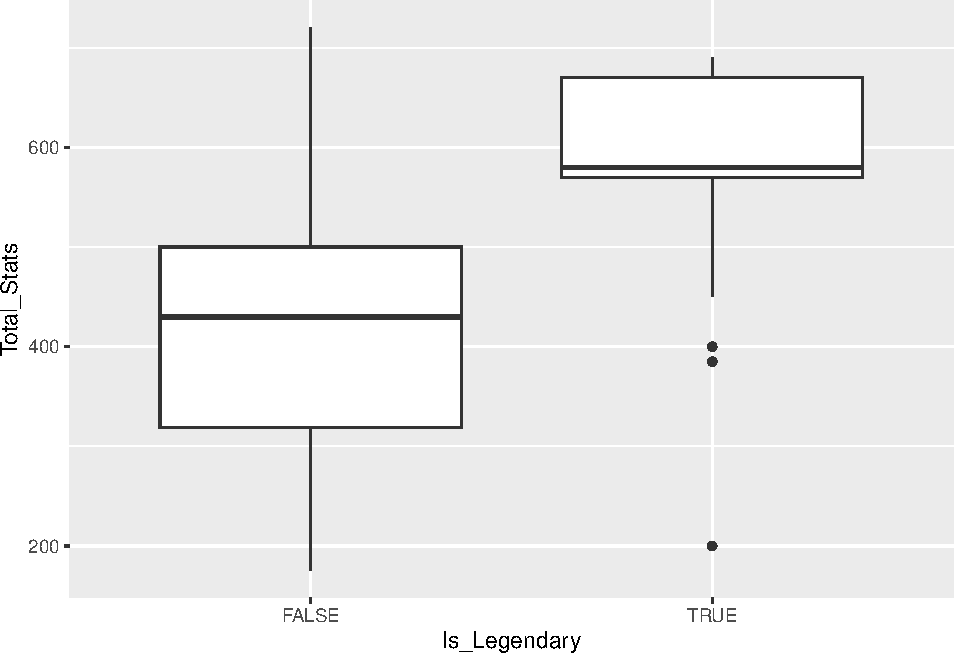
\includegraphics[width=0.9\linewidth,]{informe_files/figure-latex/unnamed-chunk-6-1} \end{center}

\subsection{podemos observar que en vista de las medidas de posición los
legendarios segun nuestras muestras siempre seran mas fuertes que los
que no son
legendarios}\label{podemos-observar-que-en-vista-de-las-medidas-de-posiciuxf3n-los-legendarios-segun-nuestras-muestras-siempre-seran-mas-fuertes-que-los-que-no-son-legendarios}

\chapter{Análisis de Resultados}

\{\small Este capítulo presenta los resultados obtenidos al aplicar las
metodologías descritas en el capítulo anterior, así como del análisis
estadístico descriptivo de las variables estudiadas y las ventajas y
desventajas al aplicar dichos tests.\}

\section{Presentación de resultados 1}

Descripción\\

\section{Presentación de resultados 2}

Descripción\\

\section{Presentación de resultados n}

Descripción\\

\chapter{Conclusiones y Recomendaciones}

\textbf{1.-} Conclusion 1 del trabajo de investigación.\\

\textbf{Recomendación} Recomendación 1 del trabajo de investigación.\\

\textbf{2.-} Conclusion 2 del trabajo de investigación.\\

\textbf{Recomendación} Recomendación 2 del trabajo de investigación.\\

\textbf{n.-} Conclusion n del trabajo de investigación.\\

\textbf{Recomendación} Recomendación n del trabajo de investigación.\\

\appendix
\renewcommand{\thechapter}{\Alph{chapter}}

\chapter{Anexo A}

\chapter{Anexo B}

\chapter{Anexo C}

%%%%%%%%%%%%%%%%%%%%%%%%%%%%%%%%%%%%%%%%%%%%%%%%%%%%%
%                   REFERENCIAS                     %
%%%%%%%%%%%%%%%%%%%%%%%%%%%%%%%%%%%%%%%%%%%%%%%%%%%%%
% Mantenemos la estructura natbib de tu plantilla
\renewcommand{\bibname}{Lista de Referencias}
\bibliographystyle{apalike} 
\bibliography{bibliografia.bib} 

%%%%%%%%%%%%%%%%%%%%%%%%%%%%%%%%%%%%%%%%%%%%%%%%%%%%%
%                   APÉNDICES                       %
%%%%%%%%%%%%%%%%%%%%%%%%%%%%%%%%%%%%%%%%%%%%%%%%%%%%%

\end{document}
